\begin{center}
    {\LARGE \textbf{2023有机化学与分析化学}} \\[2ex]
    {\large 时量180分钟 \quad 满分150分}
\end{center}

\vspace{0.5cm}
\noindent\textbf{注意事项:}
\begin{enumerate}[label=\arabic*., parsep=0pt, itemsep=0pt]
    \item 答题前,考生先将自己的姓名、学号、考场号、座位号填写在答题卡上,将条形码准确粘贴在考生信息条形码粘贴区。
    \item 考试结束后,将本试卷与答题纸一并收回。
    \item 回答各个问题时,将答案写在答题纸上,写在本试卷上无效。
\end{enumerate}

\vspace{1cm}
\begin{center}
    {\Large \textbf{有机化学部分(共100分)}}
\end{center}

\vspace{0.5cm}
\noindent\textbf{一、选择题（15 pts.）}

\begin{enumerate}[label=\arabic*., itemsep=1.5ex]
    \item 下列碳正离子中，最稳定的是
    
    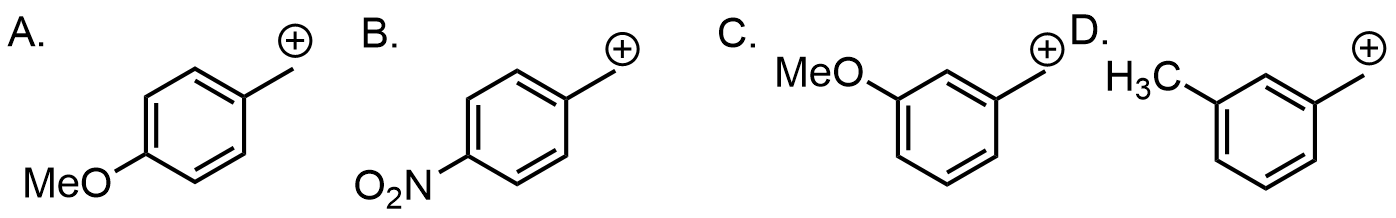
\includegraphics[scale=0.38, valign=c]{./Figure/2023/2023_4_1.png}
    \item 下列化合物不具有芳香性的是
    
    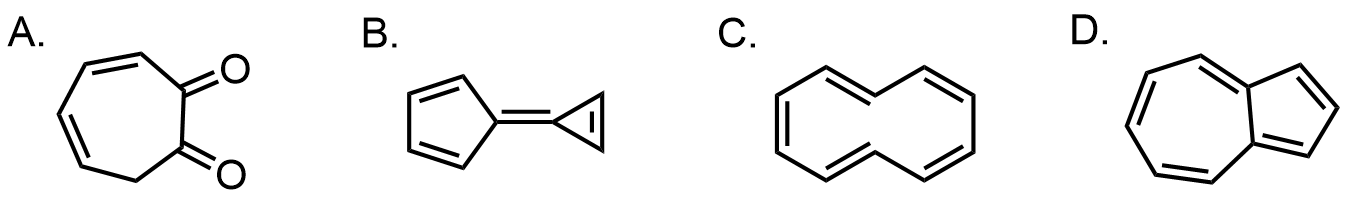
\includegraphics[scale=0.38, valign=c]{./Figure/2023/2023_4_2.png}
    \item 下列化合物中，不具有手性的分子是
    
    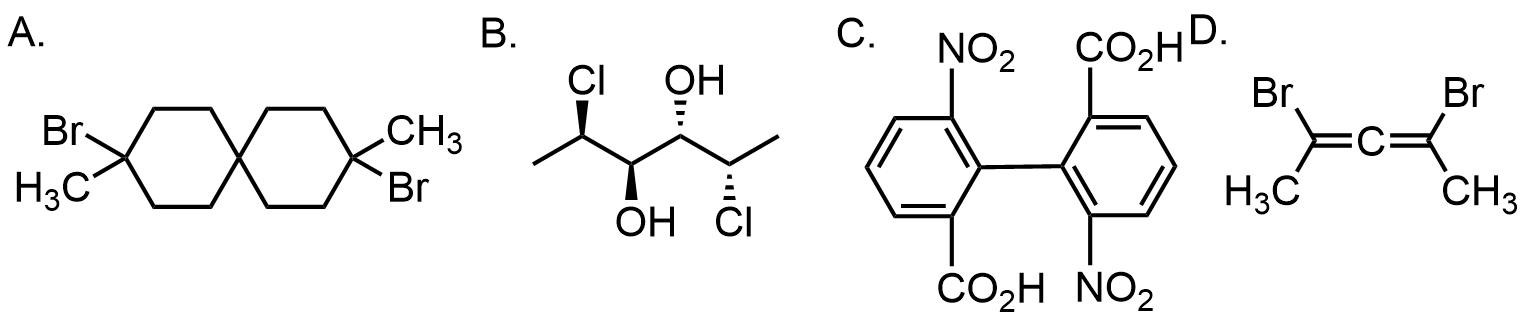
\includegraphics[scale=0.38, valign=c]{./Figure/2023/2023_4_3.png}
    \item 下列试剂中，三苯甲基醚不稳定的是
    \begin{tasks}(4)
        \task 碱
        \task Grignard试剂
        \task 烷基锂
        \task 酸
    \end{tasks}
    \item 下列试剂中，酸性最强的是
    \begin{tasks}(4)
        \task 三氯乙酸
        \task 乙酸
        \task 氯乙酸
        \task 溴乙酸
    \end{tasks}
    \item 下列化合物有其它三项结构不同的是
    
    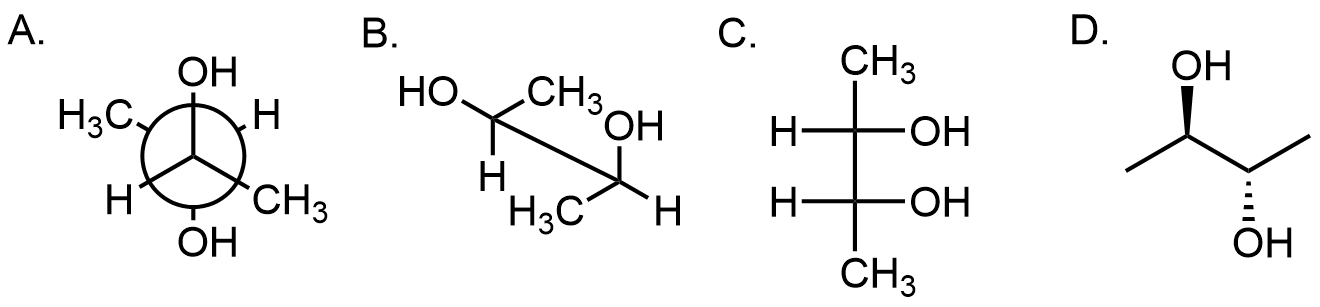
\includegraphics[scale=0.38, valign=c]{./Figure/2023/2023_4_6.png} 
    \item 下列刻意绘出的端氢中，酸性最弱的是
    
    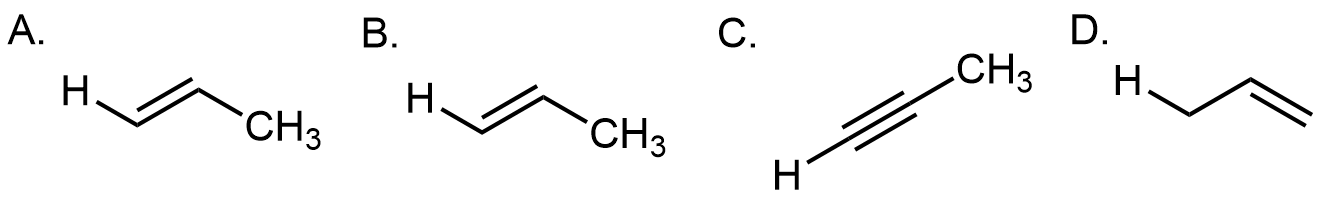
\includegraphics[scale=0.38, valign=c]{./Figure/2023/2023_4_7.png} 
    \item 下图所示分子发生单氯代反应所得同分异构体数目为
    
    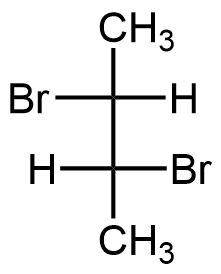
\includegraphics[scale=0.38, valign=c]{./Figure/2023/2023_4_8.png} 
    \begin{tasks}(4)
        \task 3
        \task 4
        \task 5
        \task 6
    \end{tasks}
    \item 在酸性条件下，2-甲基环己酮与等摩尔的溴单质发生反应时，将发生在哪个位置
    
    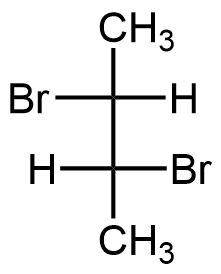
\includegraphics[scale=0.38, valign=c]{./Figure/2023/2023_4_8.png} 
    \begin{tasks}(4)
        \task 1
        \task 2
        \task 3
        \task 4
    \end{tasks}
    \item 等摩尔甲醛和苯甲醛经浓碱处理将生成
    \begin{tasks}(2)
        \task 甲醇+苯甲醇
        \task 甲酸负离子+苯甲酸负离子
        \task 苯甲酸负离子+甲醇
        \task 甲酸负离子+苯甲醇
    \end{tasks}
    \item 下列化合物的水解反应速率最快的是
    \begin{tasks}(2)
        \task \ce{CF3COOC2H5}
        \task \ce{CH3COOC2H5}
        \task \ce{CH3CH2COOC2H5}
        \task \ce{ClCH2COOC2H5}
    \end{tasks}
    \item 下列化合物中，不能和乙烯发生[4+2]环加成反应的是
    
    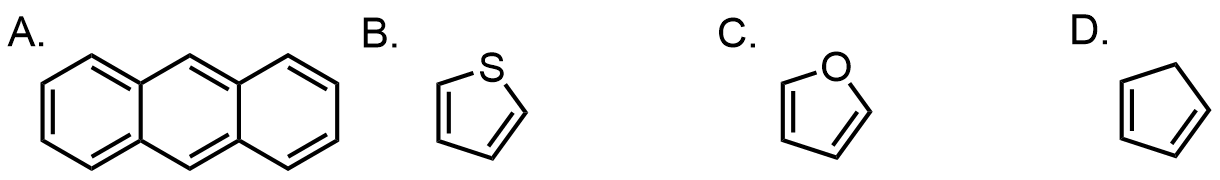
\includegraphics[scale=0.38, valign=c]{./Figure/2023/2023_4_12.png}
    \item 下列化合物不能与HCN发生反应的是
    \begin{tasks}(2)
        \task \ce{CH3CH(OH)CH2CH3}
        \task \ce{CH2ICOCH2CH3}
        \task \ce{CH3COCH2Ph}
        \task \ce{CH3OCOCH2CHO}
    \end{tasks}
    \item 下列化合物不能发生碘仿反应的是
    \begin{tasks}(4)
        \task 环己酮
        \task 苯乙酮
        \task 呋喃甲醛
        \task 2-丁酮
    \end{tasks}
    \item 下列化合物中，烯醇式含量最高的是
    \begin{tasks}(2)
        \task \ce{CH3COCH2CONH2}
        \task \ce{CH3COCH2COCH3}
        \task \ce{CH3COCH2CHO}
        \task \ce{CH3COCH2COOCH3}
    \end{tasks}
\end{enumerate}

\vspace{0.5cm}
\noindent\textbf{二、完成反应(30 pts.)}

\begin{enumerate}[label=\arabic*., itemsep=3ex]
    \item 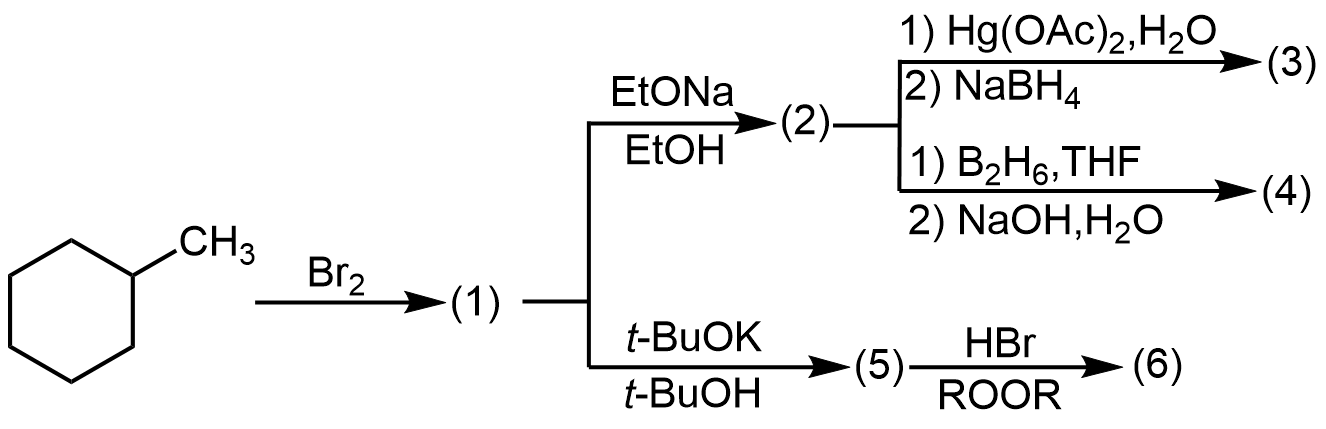
\includegraphics[scale=0.3, valign=c]{./Figure/2023/2023_1_1.png} 
    \item 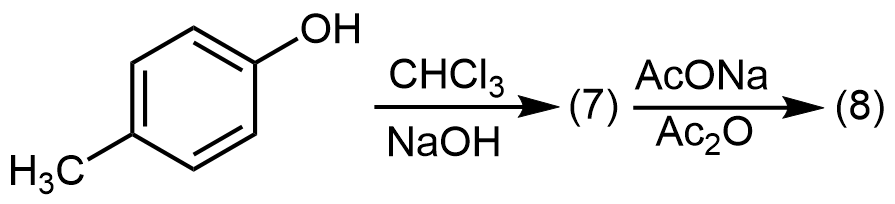
\includegraphics[scale=0.3, valign=c]{./Figure/2023/2023_1_2.png}
    \item 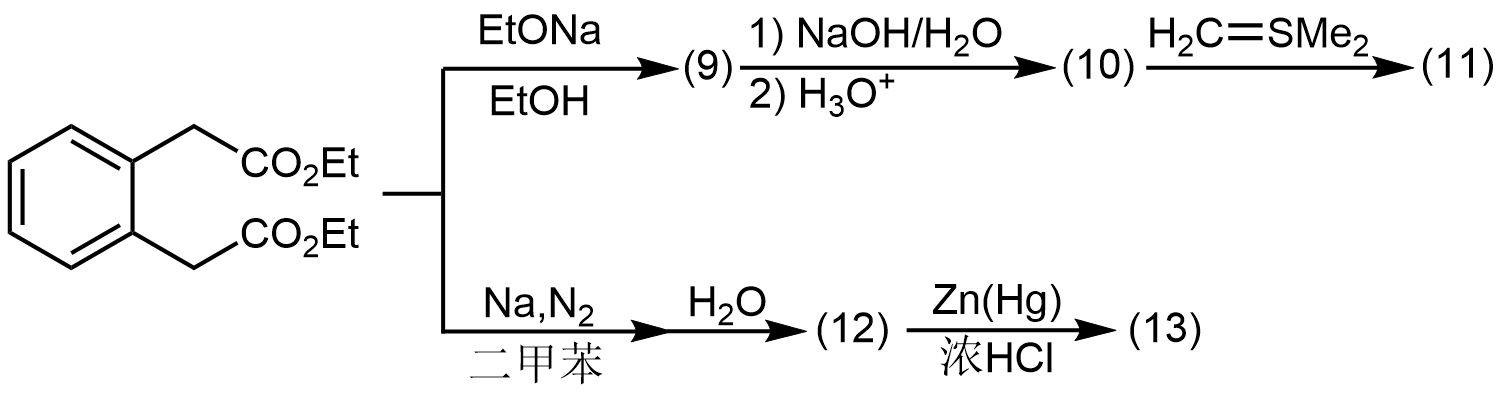
\includegraphics[scale=0.3, valign=c]{./Figure/2023/2023_1_3.png}
    \item 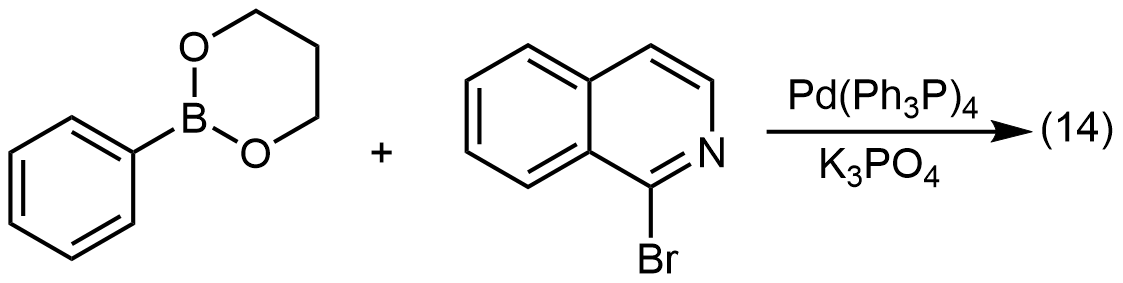
\includegraphics[scale=0.3, valign=c]{./Figure/2023/2023_1_4.png}
    \item 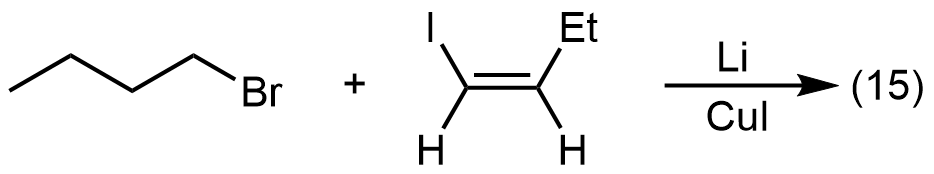
\includegraphics[scale=0.3, valign=c]{./Figure/2023/2023_1_5.png}
    \item 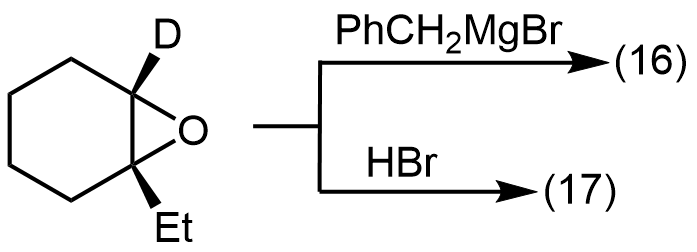
\includegraphics[scale=0.3, valign=c]{./Figure/2023/2023_1_6.png}
    \item 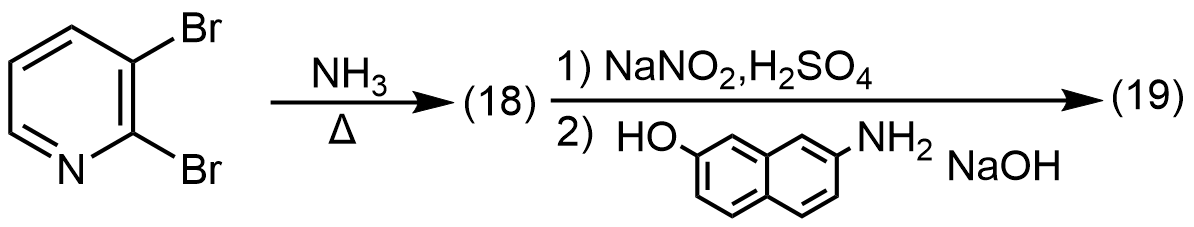
\includegraphics[scale=0.3, valign=c]{./Figure/2023/2023_1_7.png}
    \item 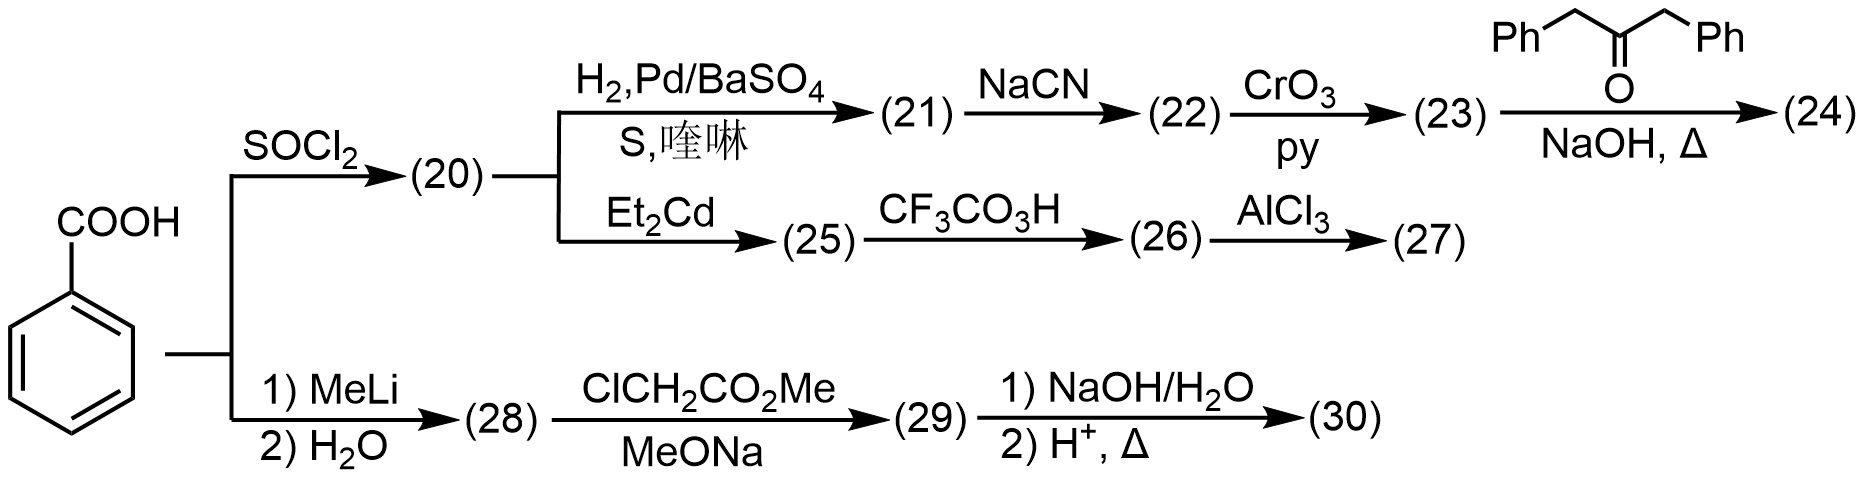
\includegraphics[scale=0.3, valign=c]{./Figure/2023/2023_1_8.png}

\end{enumerate}

\vspace{0.5cm}
\noindent\textbf{三、简答题(6 pts.)}

\begin{enumerate}[label=\arabic*., itemsep=3ex]
    \item 试解释下列化合物发生硝化反应的相对速率
    
    \begin{table}[htbp]
    \centering
        \begin{tabular}{cc}
            \toprule
            化合物 & 相对反应速率 \\
            \midrule
            硝基苯 & $6 \times 10^{-8}$ \\
            氯苯 & 0.033 \\
            苯 & 1 \\
            苯酚 & 1000 \\
            \bottomrule
        \end{tabular}
    \end{table}
\end{enumerate}


\vspace{0.5cm}
\noindent\textbf{四、机理题(14 pts.)}

\begin{enumerate}[label=\arabic*., start=1, itemsep=1.5ex]
    \item 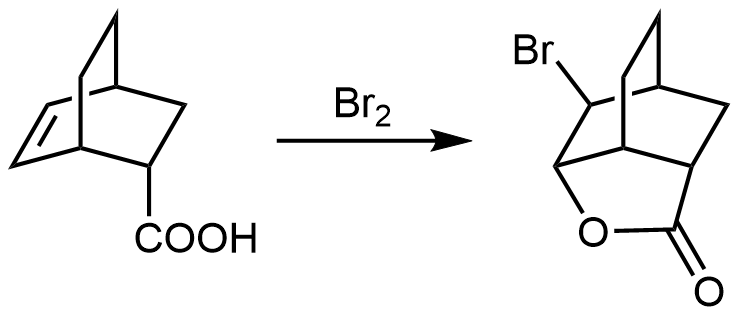
\includegraphics[scale=0.3, valign=c]{./Figure/2023/2023_2_1.png}
    \item 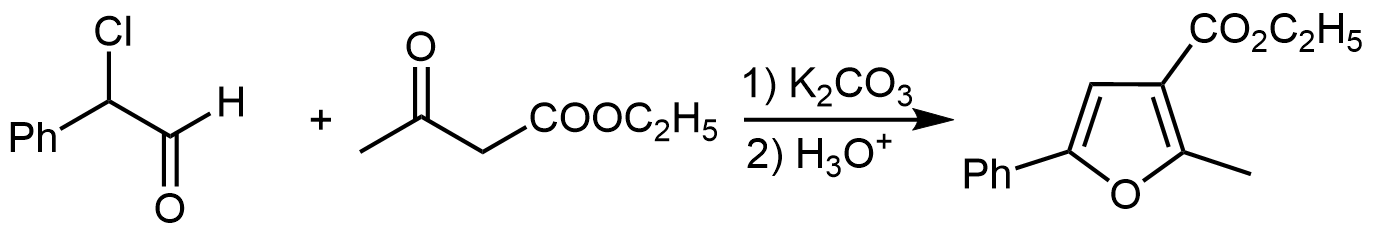
\includegraphics[scale=0.3, valign=c]{./Figure/2023/2023_2_2.png}

\end{enumerate}

\newpage

\vspace{0.5cm}
\noindent\textbf{五、合成题(35 pts.)}

\begin{enumerate}[label=\arabic*., start=1, itemsep=1.5ex]

    \begin{figure}[htbp]
        \centering
        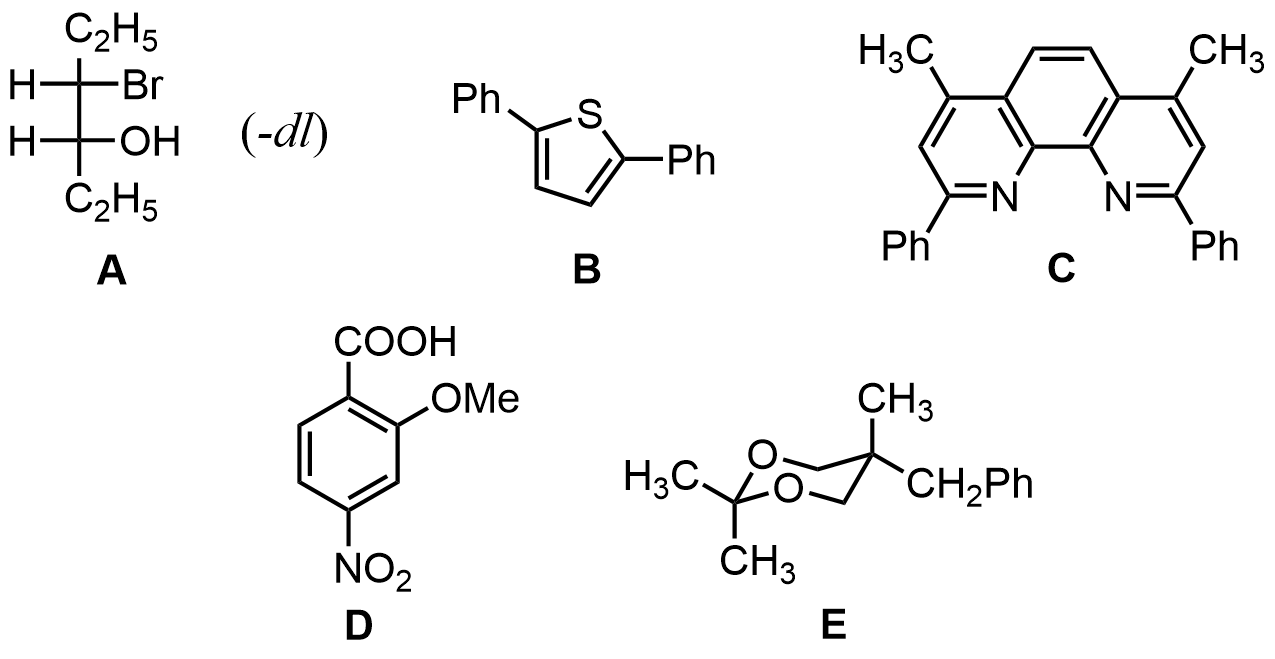
\includegraphics[scale=0.38]{./Figure/2023/2023_3.png}
    \end{figure}
    \item 以乙炔为唯一的有机原料合成\textbf{A}
    \item 以苯和小于等于2个碳的有机化合物为原料合成\textbf{B}
    \item 以苯或甲苯和小于等于3个碳的有机化合物为原料合成\textbf{C}
    \item 以苯或甲苯和小于等于2个碳的有机化合物为原料合成\textbf{D}
    \item 以苯和小于等于3个碳的有机化合物为原料合成\textbf{E}
\end{enumerate}

\vspace{1cm}
\begin{center}
    {\Large \textbf{分析化学部分(共50分)}}
\end{center}


\vspace{0.5cm}
\noindent\textbf{六、简答题}

\begin{enumerate}[label=\arabic*., itemsep=1.5ex]
    \item 根据有效数字运算规则，计算下列算式结果
    \begin{enumerate}[label=(\arabic*), noitemsep, topsep=0pt, partopsep=0pt]
        \item $11.05 + 1.3153 + 1.225 + 25.0678$
        \item 将 $3.451$ 保留两位有效数字
        \item 将 $15.3748$ 保留四位有效数字
    \end{enumerate}
    \item 已知半反应 \ce{VO2+ + 2H+ + e- = VO^{2+} + H2O} 的标准电极电位 $\varphi^\ominus=1.00\,\text{V}$，计算 $\text{pH}=2.00$ 时，溶液中电对 $\ce{VO2+/VO^{2+}}$ 的条件电位 $\varphi^\ominus{}'$。
    \item 莫尔法所用的指示剂是什么？请说明莫尔法通常在中性或弱碱性溶液中滴定的原因。
    \item 用 EDTA 在弱碱性溶液中滴定 $\ce{Cu^{2+}}$ 时，常在 \ce{NH3}-\ce{NH4+}溶液中进行，其作用是什么？
    \item 求 $\ce{CaF2}$ 在 $0.01\,\text{mol/L}\ \ce{HCl}$ 溶液中的溶解度（忽略沉淀溶解消耗的酸），已知 $K_a=10^{-3.18}$，$K_{\text{sp}}=10^{-10.57}$。
\end{enumerate}

\vspace{0.5cm}
\noindent\textbf{七、计算题}

\begin{enumerate}[label=\arabic*., itemsep=1.5ex]
    \item 用 $0.10\,\text{mol/L}$ 的 $\ce{NaOH}$ 溶液滴定 $0.10\,\text{mol/L}$ 的 $\ce{HCl}$ 溶液和 $0.20\,\text{mol/L}$ 的一元弱酸 $\ce{HA}$ 的混合溶液（已知 $K_a=5.8\times10^{-10}$）
    \begin{enumerate}[label=(\arabic*), noitemsep, topsep=0pt, partopsep=0pt]
        \item 计算化学计量点时溶液的 $\text{pH}$
        \item 若滴定终点 $\text{pH}$ 比化学计量点的 $\text{pH}$ 高 $0.5$ 个 $\text{pH}$ 单位，计算终点误差
    \end{enumerate}
    \item 浓度均为 $0.0100\,\text{mol/L}$ 的 $\ce{Zn^{2+}, Cd^{2+}}$ 混合溶液，加入过量 $\ce{KI}$，使终点时游离 $\ce{I^-}$ 浓度为 $1.0\,\text{mol/L}$，在 $\text{pH}=5.0$ 时，以二甲酚橙做指示剂，用等浓度的 EDTA 滴定其中的 $\ce{Zn^{2+}}$，计算终点误差。
    \\
    已知：$\lg K_{\ce{ZnY}}=16.50$，$\lg K_{\ce{CdY}}=10.7$，$\ce{Cd^{2+}}$ 与 $\ce{I^-}$ 形成的络合物的 $\lg\beta_1-\lg\beta_4$ 依次为 $2.10, 3.43, 4.49, 5.41$；$\text{pH}=5.0$ 时，$\text{pZn}_{\text{ep}}(\text{二甲酚橙})=4.8$，$\lg\alpha_{Y(\text{H})}=6.453$。
    \item 用一种新方法测定试样中的锌（\%），平行测定了 6 次，测得结果如下（\%）：$1.56, 1.58, 1.62, 1.60, 1.68, 1.65$，试求：
    \begin{enumerate}[label=(\arabic*), noitemsep, topsep=0pt, partopsep=0pt]
        \item 平均值的置信区间（$P=95\%$）
        \item 若已知试样中锌的标准值为 $1.68\%$，试问采用新方法后是否引起系统误差（显著性水平 $0.05$）
    \end{enumerate}

    已知：
    \begin{center}
    \begin{tabular}{|c|c|c|c|}
    \hline
    $f$ & 4 & 5 & 6 \\
    \hline
    $t_{0.05}$ & 2.78 & 2.57 & 2.45 \\
    \hline
    \end{tabular}
    \end{center}
\end{enumerate}